\subsection{深度学习(神经网络)}
\subsubsection{多层感知机}
\begin{frame}
    \frametitle{Why Neural Networks Can Learn Almost Anything\footnote{\href{https://www.youtube.com/watch?v=0QczhVg5HaI}{youtube视频}}}
    函数是抽象现实世界的好方法,如 \(\displaystyle F=G\frac{Mm}{R^2}\),
    但是我们经常遇到的是并不知道函数的解析形式而只知道某几个点或者某一段的值。
    计量里面我们学过用 OLS 把样本点拟合成一个线性函数,神经网络是源于对生物神经的模拟,是一种通用的函数估计方法\cite{hornik1989multilayer}。
    \begin{figure}[hb]
        \href{https://playground.tensorflow.org/}{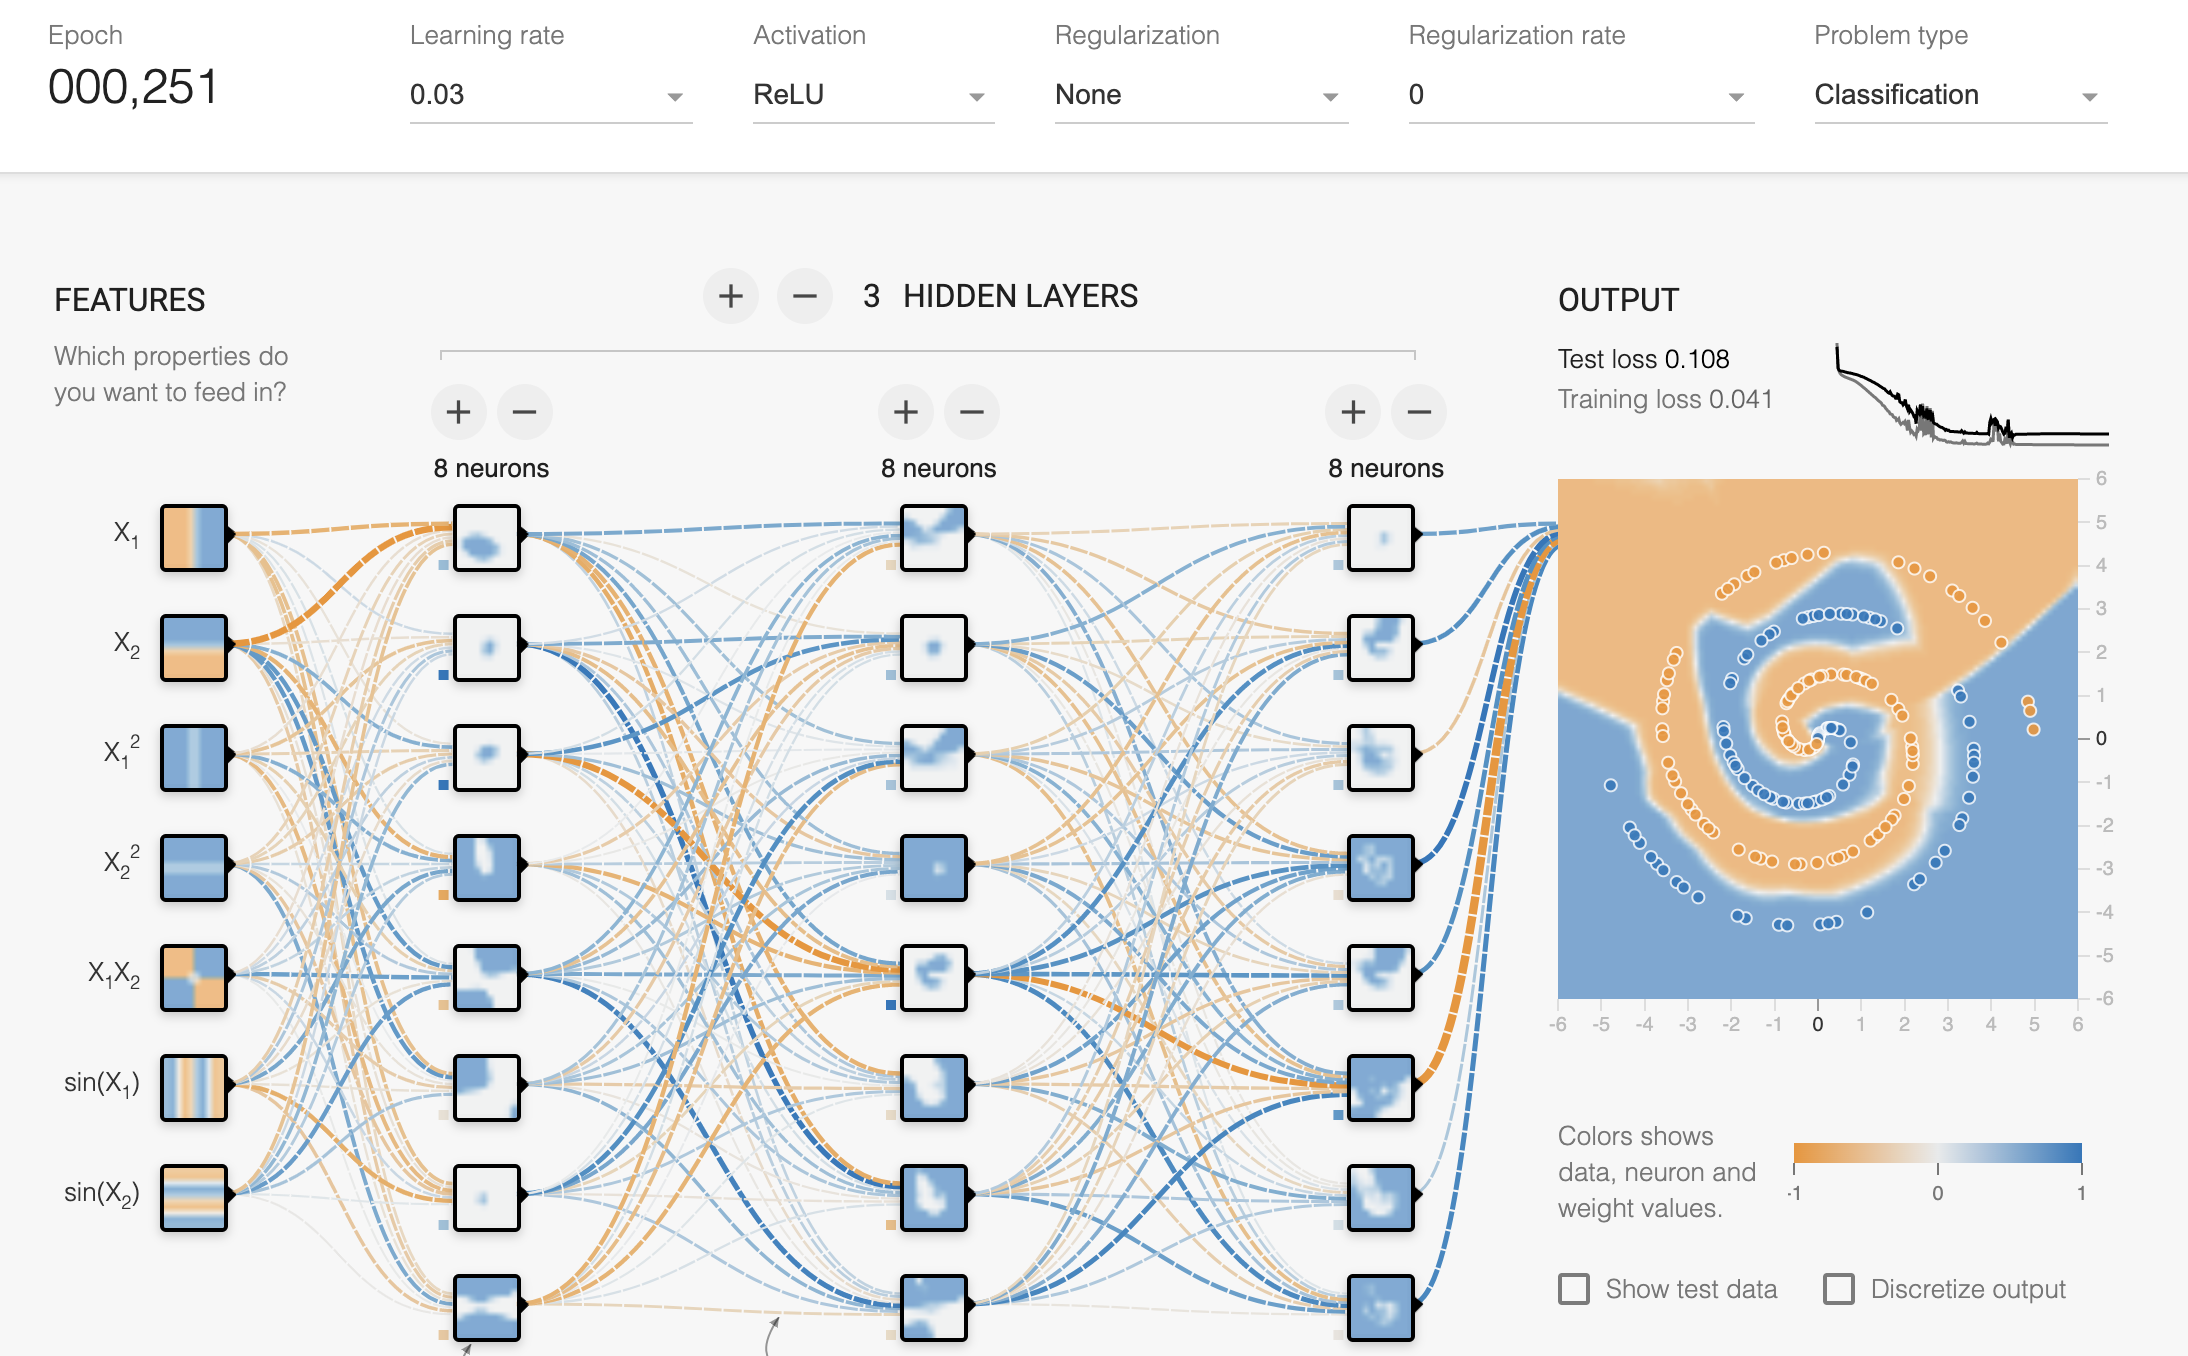
\includegraphics[width=0.7\linewidth]{../lib/tfplay.png}}
    \end{figure}
\end{frame}
\begin{frame}
    \frametitle{图的含义}
    在坐标轴上,蓝色代表该位置值为 1,橙色为 -1。我们通过 $x_1$ $x_2$ 的组合来拟合真实的 Y (右图 output 的散点)。
    \only<1>{拟合的方式为
        \begin{eqnarray}
            Y&=& Activation(X_1,X_2)\nonumber\\
            Linear(X_1,X_2) &=& b_1X_1+b_2X_2\nonumber
        \end{eqnarray}
    }
    \only<2>{一层输出作为另一层输入的“网络”
        \begin{eqnarray}
            Y_i&=& Linear(X_1,X_2)\nonumber\\
            Y(Y_1,Y_2) &=& Linear(Y_1,Y_2)\nonumber
        \end{eqnarray}
    }
    \only<3>{线性函数再怎么叠加,其结果仍然是线性的
        \begin{eqnarray}
            H_i&=& Linear(I_j,I_k) \nonumber\\
            Y &=& b_1X_1+b_2X_2\nonumber
        \end{eqnarray}
    }
    \only<1>{
        \begin{figure}[hb]
            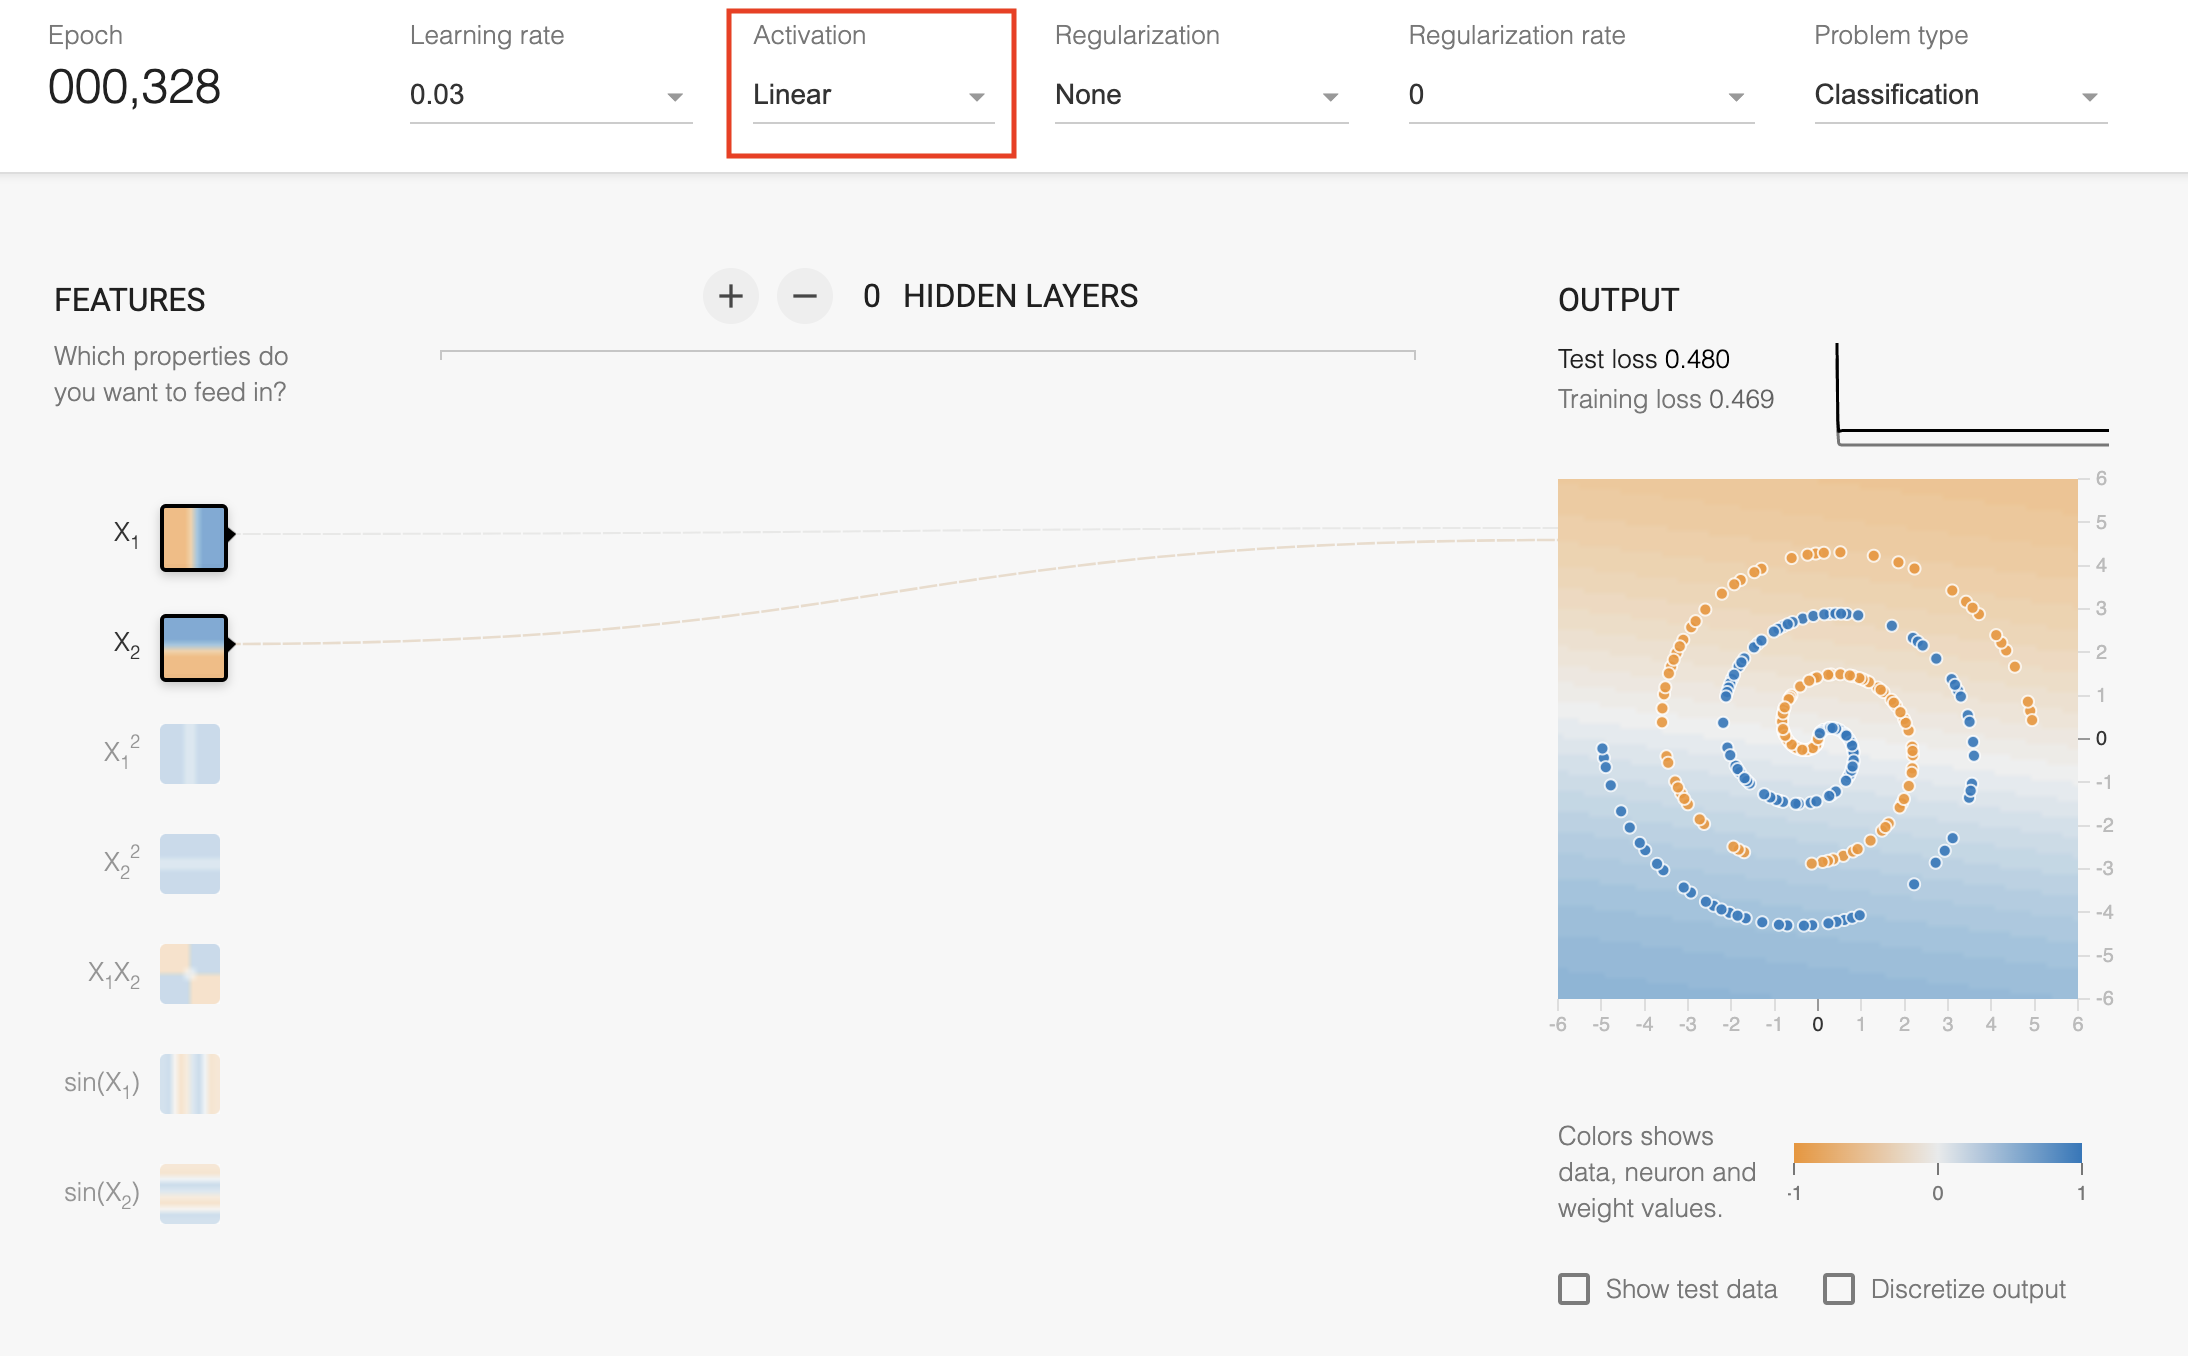
\includegraphics[width=0.7\linewidth]{../lib/init.png}
        \end{figure}
    }
    \only<2>{
        \begin{figure}[hb]
            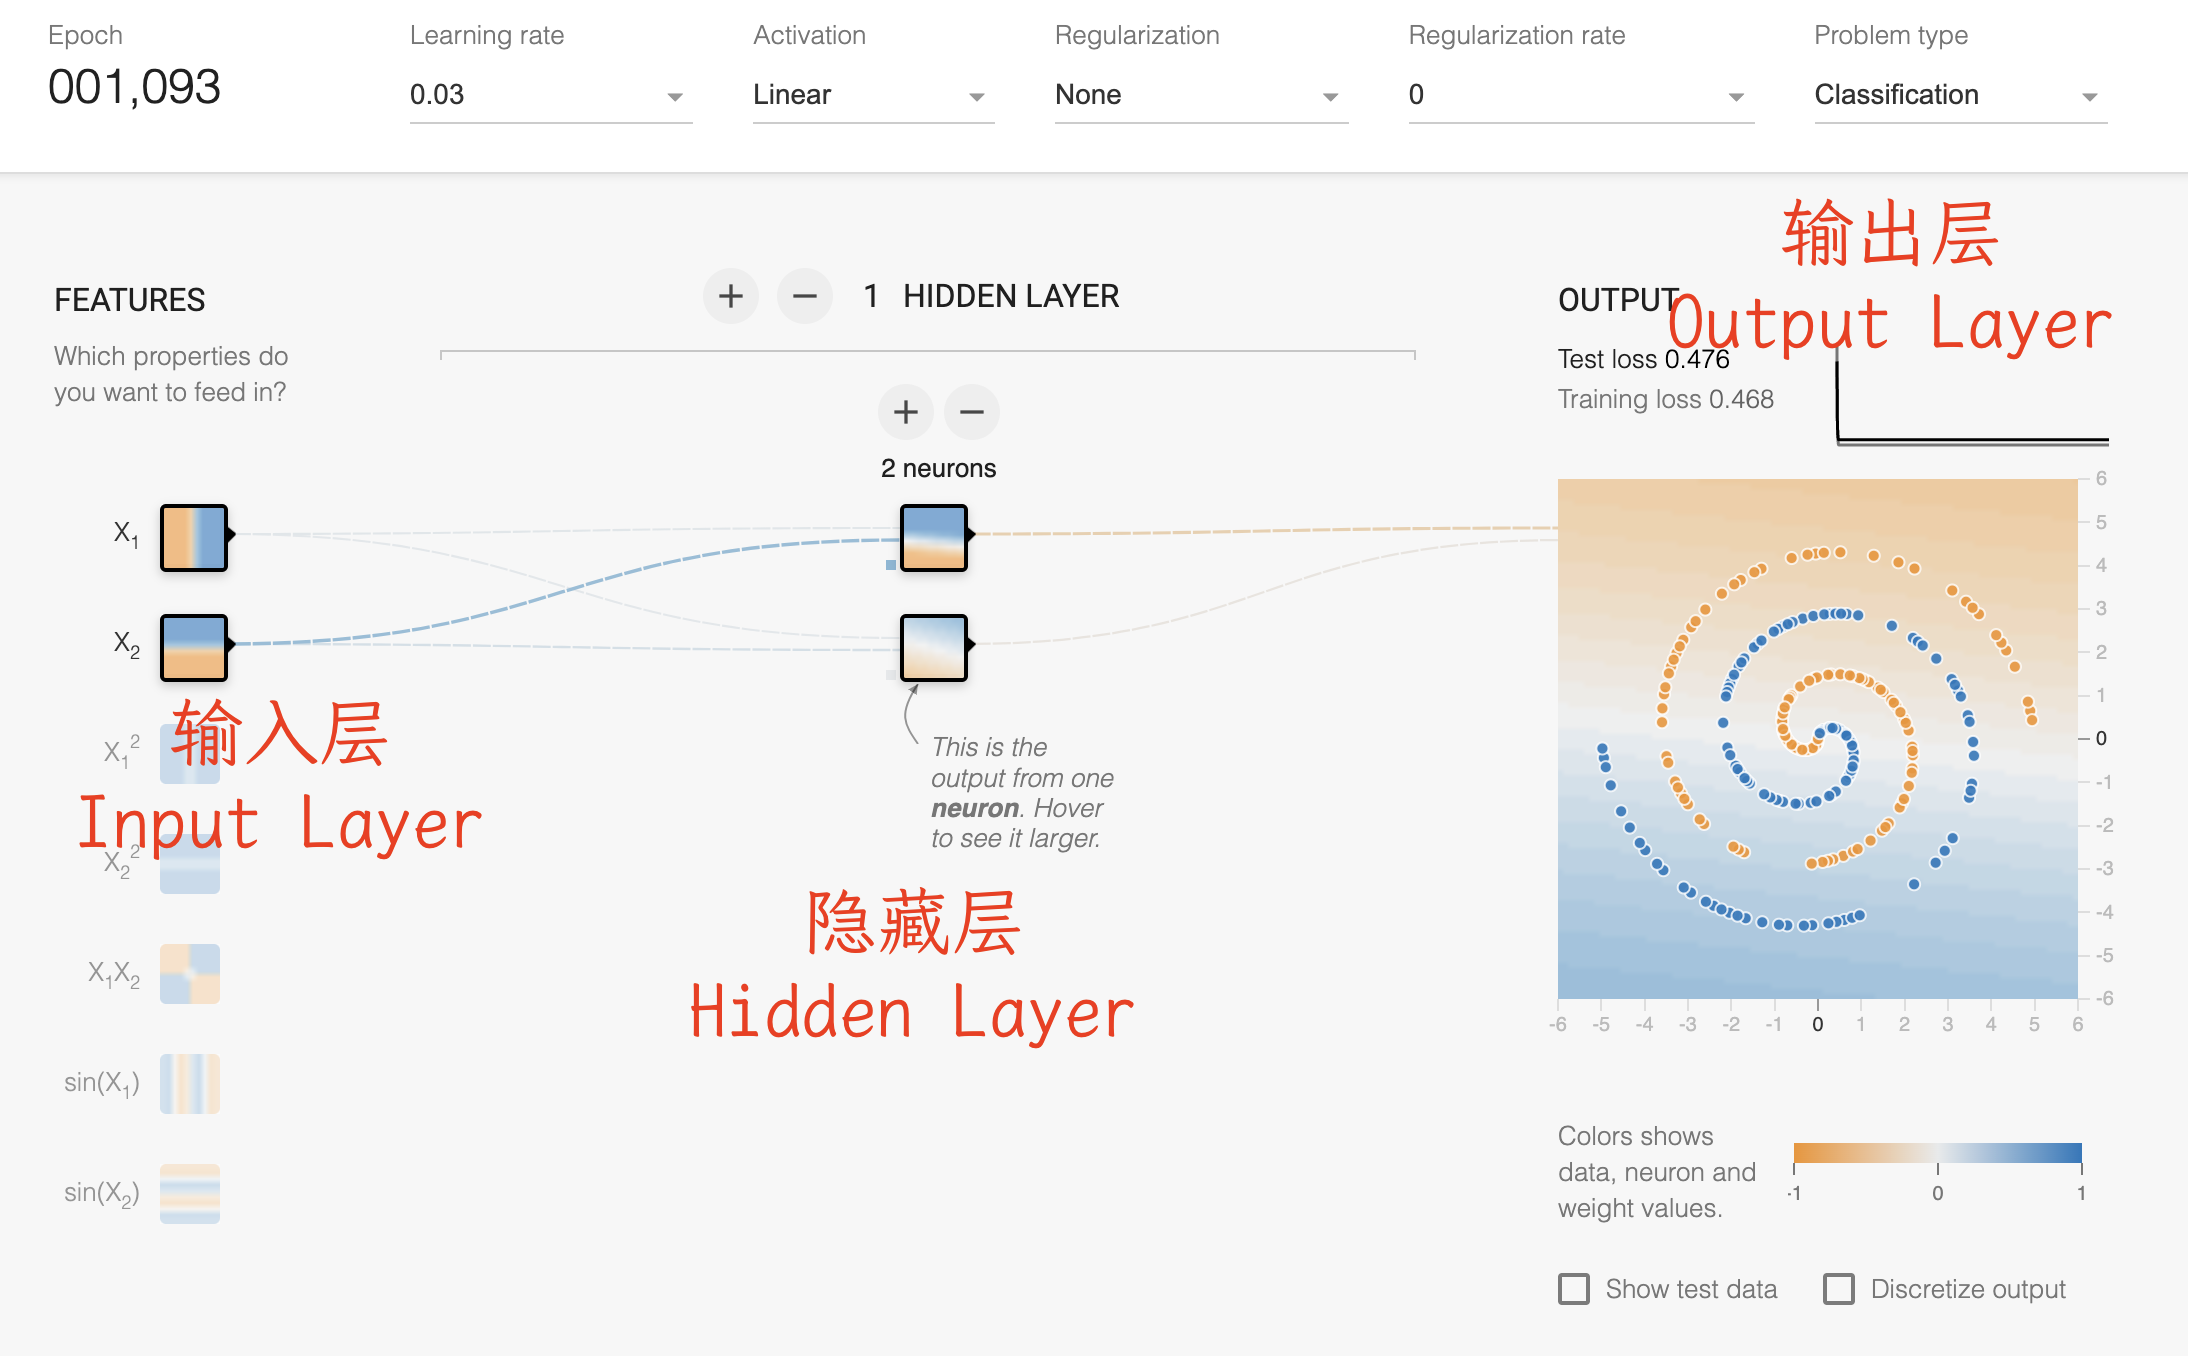
\includegraphics[width=0.7\linewidth]{../lib/initwithnet.png}
        \end{figure}
    }
    \only<3>{
        \begin{figure}[hb]
            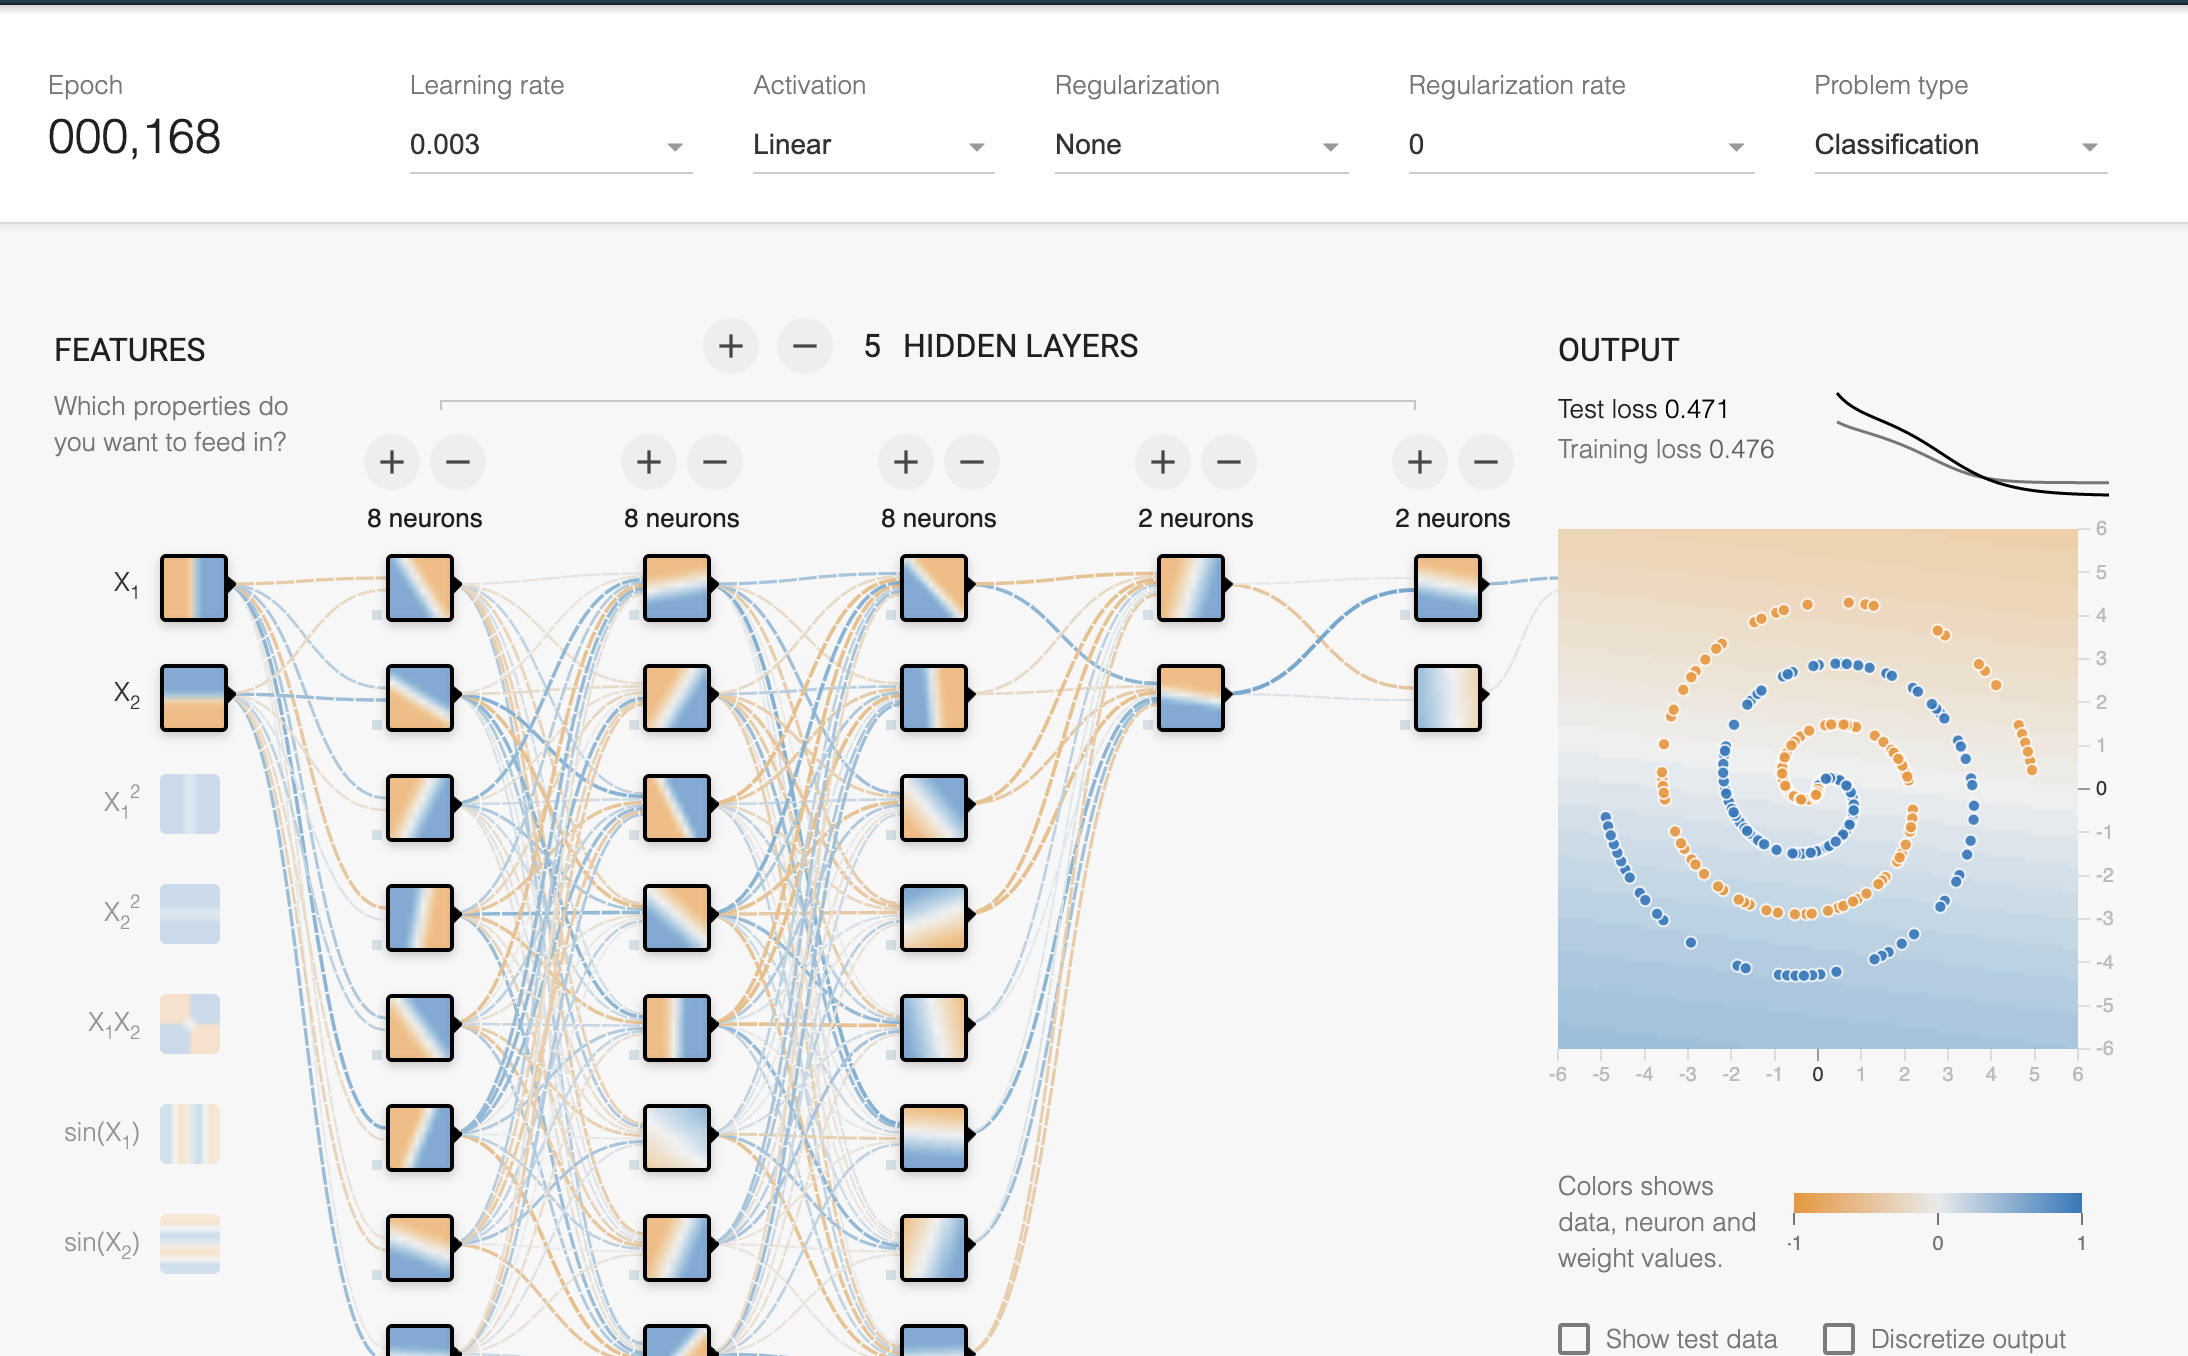
\includegraphics[width=0.7\linewidth]{../lib/initwithhugenet.png}
        \end{figure}
    }
\end{frame}
\begin{frame}
    \frametitle{激活函数}
    \begin{columns}
        \column{0.5\linewidth}
        \begin{figure}

            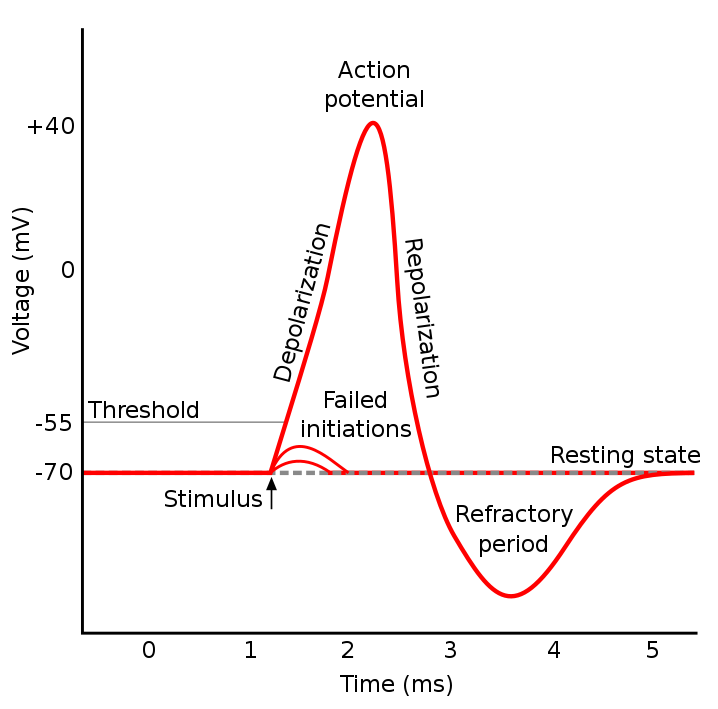
\includegraphics[width=\linewidth]{../lib/neuron.png}
            \caption{生物神经的动作电位}
        \end{figure}

        \column{0.5\linewidth}
        线性函数的叠加仍然是线性函数。

        为了实现对非线形特征的识别,也为了对生物神经有更好的模拟,神经网络中每个神经元的输入添加了非线性的“\textbf{激活
            函数}”。常见的有:

        \begin{eqnarray}
            ReLU(x)&=&\max(0,x)\\
            Sigmoid(x)&=&\frac {1}{1+e^{-x}}\\
            tanh(x)&=&\tanh{x}\\
            Softmax(x_i)&=&\frac{e^{x_i}}{\sum e^{x_j}}
        \end{eqnarray}
        % 利用激活函数,神经网络可以拟合出任意的函数,而多层的神经网络在拟合时更有效率
    \end{columns}
\end{frame}
\begin{frame}
    \frametitle{激活函数}
    当我们把激活函数设置成非线性的函数,如 $ReLU$,机器开始学习到了非线性的因素。
    \only<1>{
        \begin{figure}[hb]
            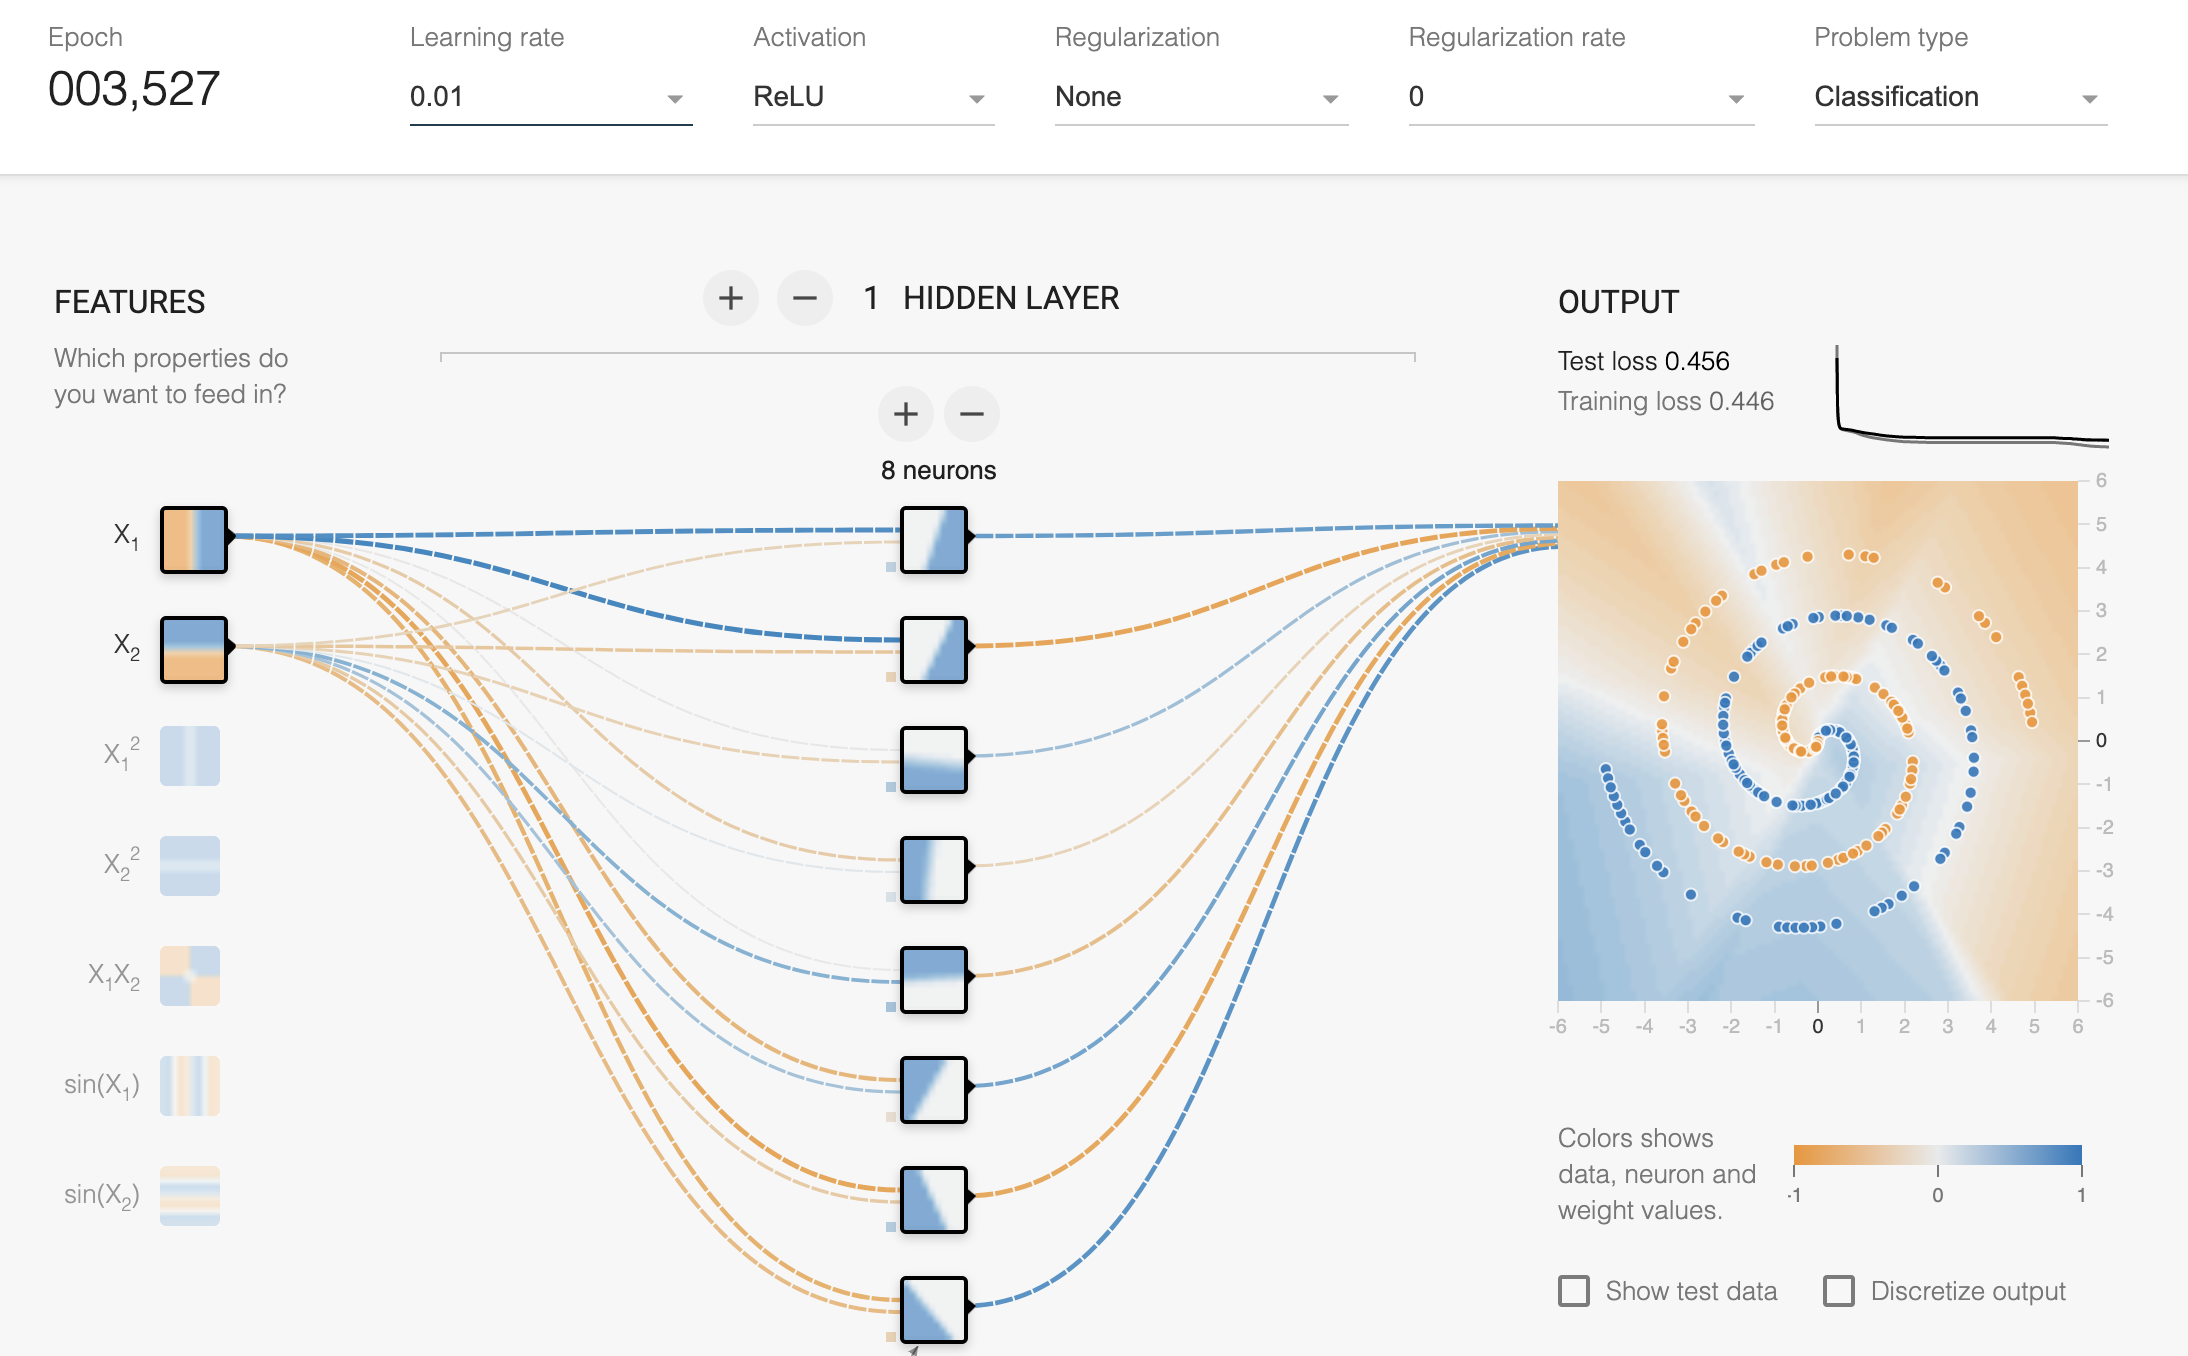
\includegraphics[width=0.7\linewidth]{../lib/relu.png}
        \end{figure}
    }
    \only<2>{
        如期权($ReLU$)这些“尖角”的组合,可以拟合任意的payoff(函数)
        \begin{figure}[hb]
            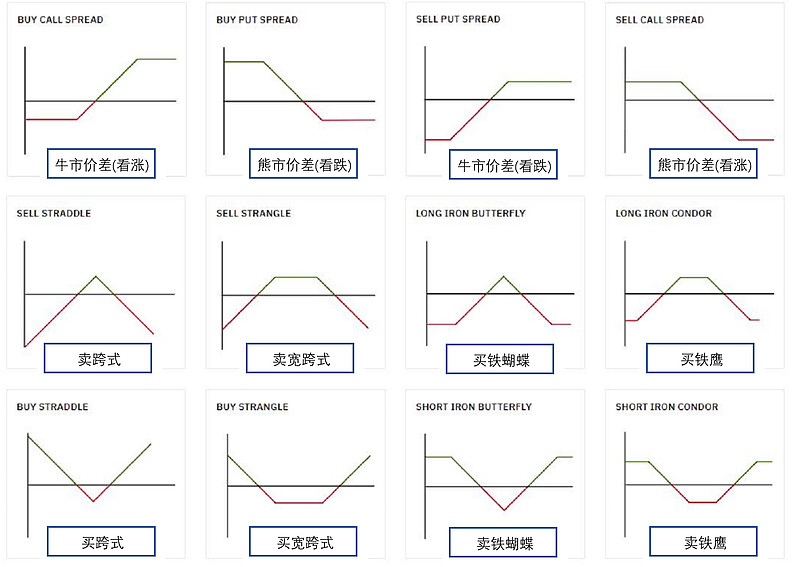
\includegraphics[width=0.7\linewidth]{../lib/options.jpeg}
        \end{figure}
    }
\end{frame}
\begin{frame}
    \frametitle{网络}
    利用激活函数,一层神经网络可以拟合出任意的函数。
    在实践过程中,人们发现多层的神经网络在拟合时更有效率
    \begin{figure}[hb]
        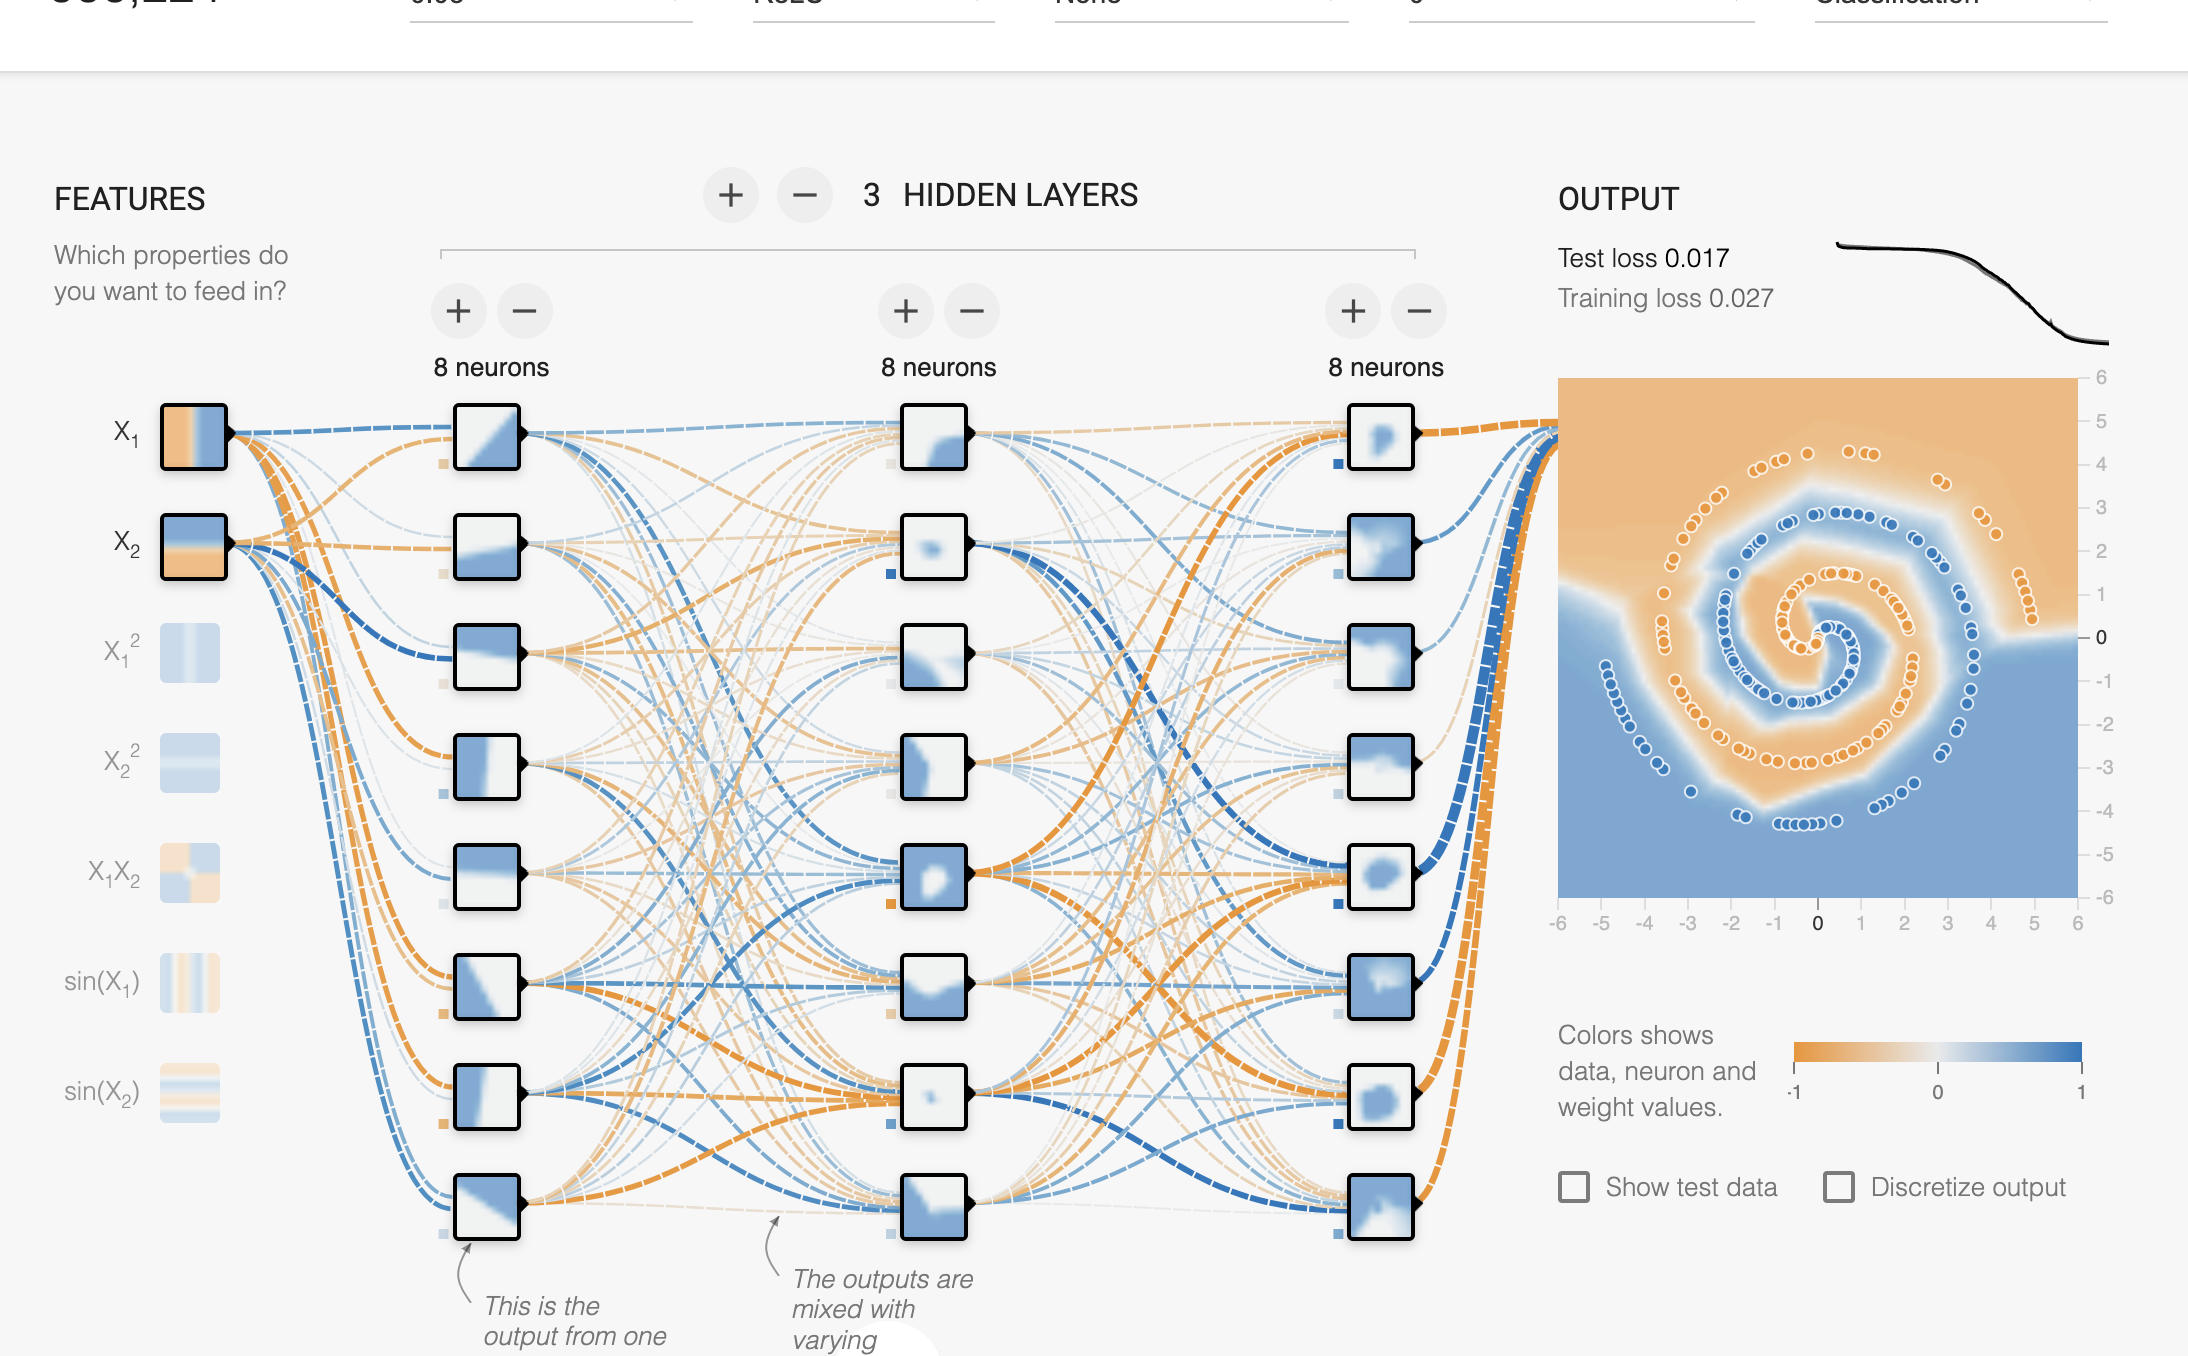
\includegraphics[width=0.7\linewidth]{../lib/final.png}
    \end{figure}
\end{frame}
\begin{frame}
    \frametitle{梯度下降与反向传播}
    \begin{columns}
        \column{0.5\linewidth}
        \begin{figure}
            \centering
            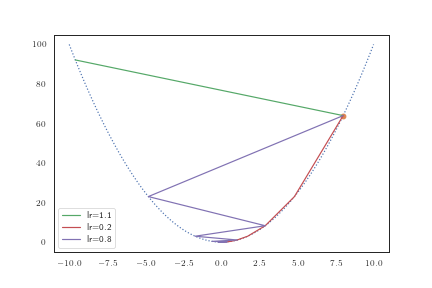
\includegraphics[width=\linewidth]{../lib/lr.png}
            \label{learningrates}
            \caption{不同学习率的影响}
        \end{figure}
        \column{0.5\linewidth}
        再进一步了解前,我们先了解一下机器是怎么样优化参数的。
        先看最简单的线性的情况。
        假设有一个我们不知道 $w,b$ 的线性的 $y=wx+b$ ,仅知道若干个 $(x,y)$。

        首先定义 \textbf{损失函数} 为 $loss = \sum{(\hat{y}-y)^2}$ ,即 $loss(w, b)=\sum(wx+b-y)^2$ 。我们目标是最小化估计的损失函数。

        令 $w=w_0,b=b_0$ ,正向计算得到 $loss(w_0,b_0)$。
        为了最小化它,我们让 $w,b$ 沿着 $loss$ 的梯度走一小步(\textbf{learning rate}),即误差反向传播。
        不断迭代,逼近 $loss(w,b)$ 的最小值,得到估计的 $w^*,b^*$。
    \end{columns}
\end{frame}

\begin{frame}[fragile]
    \frametitle{梯度下降与反向传播}
    左边的代码是我们手动实现的上述过程,右边的代码是更加 pytorch 风格的代码。
    \begin{columns}
        \column{0.5\linewidth}
        \tiny
        \begin{minted}{python}
import torch
x = torch.rand([500,1]) # 张量可以当成是特殊的向量
y_true = 3*x+8
learning_rate = 0.05
# w b 自动求导
w = torch.tensor([[0]], requires_grad=True)
b = torch.tensor(0, requires_grad=True
                    , dtype=torch.float32)
for i in range(500):
    y_pred = torch.matmul(x,w)+b # 预测值
    loss = (y_true-y_pred).pow(2).mean() # loss(w, b)
    if w.grad is not None: # 不清零会累加
        w.grad.data.zero_()
    if b.grad is not None:
        b.grad.data.zero_()
    loss.backward() # 反向传播得到梯度
    w.data = w.data - w.grad*learning_rate
    b.data = b.data - b.grad*learning_rate
    if i % 50 == 0:
        print(w.item(), b.item(), loss.item())
\end{minted}
        \column{0.5\linewidth}
        \tiny
        \begin{minted}{python}
import torch
from torch import nn,optim
class Lr(nn.Module):
    def __init__(self):
        super(Lr, self).__init__()
        self.layer = nn.Linear(1,1)
    def forward(self, x):
        return self.layer(x)
x = torch.rand([500,1])
y = 3*x+8
model = Lr()
criterion = nn.MSELoss()
optimizer = optim.SGD(model.parameters(), lr=0.05)
for i in range(500):
    out = model(x)
    loss = criterion(y, out)
    optimizer.zero_grad()
    loss.backward()
    optimizer.step()
list(model.parameters())
        \end{minted}
    \end{columns}
\end{frame}

\begin{frame}[fragile]
    \frametitle{神经网络}
    一层神经元的输出,作为另一层神经网络的输入,就形成了一层神经网络。多层神经网络通过损失函数和优化器迭代训练,就形成了一个简单的感知机。

    \begin{columns}
        \column{0.5\linewidth}
        \tiny
        \begin{minted}{python}
from torch import nn
import torch
Ytrain_nn = torch.tensor(pd.get_dummies(Ytrain).values,
                dtype=torch.float32)
Xtrain_nn = torch.tensor(Xtrain.values, dtype=torch.float32)
net = nn.Sequential(
    nn.Linear(Xtrain_nn.shape[1], 40),
    nn.ReLU(),
    nn.Linear(40, 7),
    nn.Softmax(dim=1)
)
optimizer = torch.optim.SGD(net.parameters(), lr=0.001)
loss_func = torch.nn.MSELoss()
for t in range(10000):
    prediction = net(Xtrain_nn)
    loss = loss_func(Ytrain_nn, prediction)
    optimizer.zero_grad()
    loss.backward()
    optimizer.step()
Xtest_nn = torch.tensor(Xtest.values, dtype=torch.float32)
prediction = pd.DataFrame(net(Xtest_nn).detach().numpy())
        \end{minted}
        \column{0.4\linewidth}
        \begin{table}
            \caption{感知机结果}
            \begin{tabular}{ll}
                precision & 0.3035 \\
                recall    & 0.3267 \\
                f1        & 0.2913 \\
                \(R^2\)   & 0.0463 \\
            \end{tabular}
            \label{BP}
        \end{table}
    \end{columns}
\end{frame}
\subsubsection{CNN}
\begin{frame}
    \frametitle{卷积}
    \begin{definition}{卷积}
        \begin{equation}
            (f*g)(t)=\int_{\mathbb{R}^n}f(\tau)g(t-\tau)\mathrm{d}\tau
        \end{equation}
    \end{definition}

        \begin{figure}
            \includegraphics[width=0.5\linewidth]{../lib/CNN.jpeg}
            \caption{卷积}
            \label{CNN}
        \end{figure}

\end{frame}
\begin{frame}
    \frametitle{卷积}
    卷积神经网络最早应用在图像识别领域,利用“做卷积”扫描图像上的 (R,G,B) 元组得到像素点附近的一层特征。

    \begin{tabular}{cccc}
        
\includegraphics[width=0.2\linewidth]{../lib/aniya.jpeg} & 
\includegraphics[width=0.2\linewidth]{../lib/blur.jpeg} & 
\includegraphics[width=0.2\linewidth]{../lib/sharpen.jpeg} & 
\includegraphics[width=0.2\linewidth]{../lib/dark.jpeg} \\
        original image                                           & $\begin{pmatrix}
                                                                            1 & 1 & 1 \\
                                                                            1 & 0 & 1 \\
                                                                            1 & 1 & 1
                                                                        \end{pmatrix}$                                        & $\begin{pmatrix}
                                                                                                                                     0  & -1 & 0  \\
                                                                                                                                     -1 & 5  & -1 \\
                                                                                                                                     0  & -1  & 0
                                                                                                                                 \end{pmatrix}$                                           & $\begin{pmatrix}
                                                                                                                                                                                                 -1 & 0 & 1 \\
                                                                                                                                                                                                 -1 & 0 & 1 \\
                                                                                                                                                                                                 -1 & 0 & 1
                                                                                                                                                                                             \end{pmatrix}$
    \end{tabular}
        扫描出来细致的的特征可能会导致过拟合,扫描的结果会经过“pooling”的过程减少参数和计算量,防止过拟合,提高模型泛化能力。
        最后通过一层全连接层将CNN的结果输出出来。
\end{frame}
\begin{frame}[fragile]
    \frametitle{实现 CNN}
    \begin{columns}
        \column{0.6\linewidth}
        \begin{minted}{python}
class CNN(nn.Module):
    def __init__(self) -> None:
        super(CNN, self).__init__()
        self.conv = nn.Sequential(
            nn.Conv1d(48, 20, 3,padding=2),
            nn.Tanh(),
            nn.AvgPool1d(3),
        )
        self.fc = nn.Sequential(
            nn.Linear(20, len(encode)),
            nn.ReLU(),
            nn.Softmax(dim=1),
        )

    def forward(self, x):
        out = self.conv(x).view(out.size(0), -1)
        return self.fc(out)
        \end{minted}
        \column{0.3\linewidth}
        \begin{table}
            \caption{CNN 结果}
            \begin{tabular}{ll}
                precision & 0.4027 \\
                recall    & 0.4350 \\
                f1        & 0.4140 \\
                \(R^2\)   & 0.4039 \\
            \end{tabular}
            \label{CNNres}
        \end{table}
    \end{columns}
\end{frame}
\subsubsection{RNN}
\begin{frame}
    \frametitle{“记忆”}
    在一些和时序有关的应用场景中,需要一定的记忆功能。比如翻译末尾的句子可能会参考到开头的语句。

    RNN 利用权值共享、自我更新,实现了类似“记忆”的功能。
    \begin{figure}
        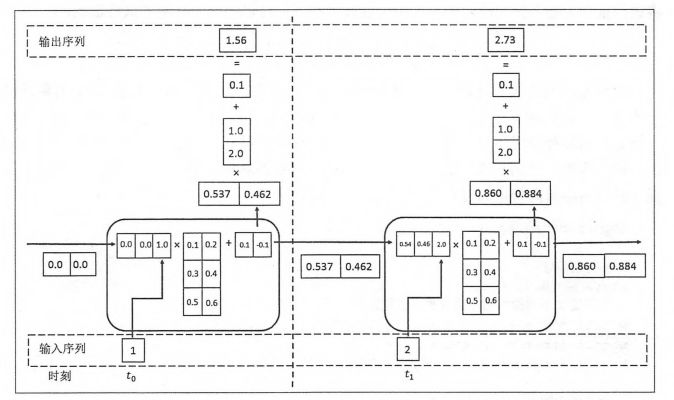
\includegraphics[width=0.6\linewidth]{../lib/RNN.jpeg}
        \caption{RNN 示意图}
        \label{RNN}
    \end{figure}
\end{frame}
\begin{frame}[fragile]
    \frametitle{实现 RNN}
    \begin{columns}
        \column{0.6\linewidth}
        \begin{minted}{python}
class RNN(nn.Module):
    def __init__(self):
        super(RNN, self).__init__()
        self.rnn = nn.RNN(
            input_size=48,
            hidden_size=100,
            batch_first=True,
        )
        self.fc = nn.Sequential(
            nn.Linear(100, len(encode)),
            nn.ReLU(),
            nn.Softmax(dim=1),
        )

    def forward(self, x):
        out, _ = self.rnn(x)
        return self.fc(out[:, -1, :])
        \end{minted}
        \column{0.3\linewidth}
        \begin{table}
            \caption{RNN 结果}
            \begin{tabular}{ll}
                precision & 0.4516 \\
                recall    & 0.4606 \\
                f1        & 0.4541 \\
                \(R^2\)   & 0.4176 \\
            \end{tabular}
            \label{RNNres}
        \end{table}
    \end{columns}
\end{frame}
\begin{frame}
    \frametitle{其他神经网络}
    \begin{itemize}
        \item CNN 的扩展:ResNet……
        \item RNN 的扩展:LSTM……
        \item \textbf{Transformer}:Attention Is All You Need
        \item GAN 生成对抗网络:机器不仅可以回归/分类,还可以创造
        \item Self-Supervised Model:仅需标注少量数据甚至不标注
        \item RL 强化学习:Alpha Go
    \end{itemize}
\end{frame}
